\documentclass[twocolumn, 9pt]{article}

\usepackage[margin=0.8in,bottom=1.25in,columnsep=.4in]{geometry}
\usepackage{amsmath}
\usepackage{amssymb}
\usepackage{listings}
\usepackage{color}
\usepackage{cite}
\usepackage{multicol}
\usepackage{graphicx}

\title{
	50.039 Theory and Practice of Deep Learning\\
	Theory Homework 4
}

\author{Joel Huang 1002530}
\date{\today}

\begin{document}
\maketitle

\section{Sigmoid function}
\subsection*{Derivative of the sigmoid function}
\begin{equation*}
	\varphi(x) = \dfrac{1}{1+e^{-ax}}
\end{equation*}
\begin{equation*}
	\varphi(x) = (1+e^{-ax})^{-1}
\end{equation*}
\begin{equation*}
	\dfrac{d\varphi}{dx} = (-1)(1+e^{-ax})^{-2}(-ae^{-ax})
\end{equation*}
\begin{equation*}
	\dfrac{d\varphi}{dx} = \dfrac{ae^{-ax}}{(1+e^{-ax})^2}
\end{equation*}
\begin{equation*}
	\dfrac{d\varphi}{dx} = a\varphi(x)\cdot \dfrac{1+e^{-ax}-1}{1+e^{-ax}}
\end{equation*}
\begin{equation*}
	\dfrac{d\varphi}{dx} = a\varphi(x)\cdot (1-\dfrac{1}{1+e^{-ax}})
\end{equation*}
\begin{equation*}
	\dfrac{d\varphi}{dx} = a\varphi(x)\cdot (1-\varphi(x))
\end{equation*}

\subsection*{Value of derivative at $x=0$}
\begin{equation*}
	\varphi(0) = \dfrac{1}{2}
\end{equation*}
\begin{equation*}
	\varphi'(0) = a\varphi(0)\cdot (1-\varphi(0))
\end{equation*}
\begin{equation*}
	\varphi'(0) = \dfrac{a}{4}
\end{equation*}

\section{Neural network layers}
\subsection*{Output of a neural network}
The output of the neural network is fed by three inputs, $h_1, h_2, w_7$.
\begin{equation*}
	output = g(w_8h_1 + w_9h_2 + w_7)
\end{equation*}
The hidden layers are fed by two inputs, $x_1, x_2$ and a bias each, scaled by the constant $c$.
\begin{equation*}
\begin{split}
	h_1 = c\cdot(w_3x_1 + w_5x_2 + w_1)\\
	h_2 = c\cdot(w_4x_1 + w_6x_2 + w_2)
\end{split}
\end{equation*}
Rearranging,
\begin{equation*}
\begin{split}
	output = g\,(&w_8c\cdot(w_3x_1 + w_5x_2 + w_1) + \\
	&w_9c\cdot(w_4x_1 + w_6x_2 + w_2) + w_7)
\end{split}
\end{equation*}
Expressing it in sigmoid form,
\begin{equation*}
	output = \dfrac{1}{1+e^{-(w_8c(w_3x_1 + w_5x_2 + w_1) + w_9c(w_4x_1 + w_6x_2 + w_2) + w_7)}}
\end{equation*}

\subsection*{Equation for a binary decision boundary at $g=0.5$}
\begin{equation*}
	\dfrac{1}{1+e^{-(w_8c(w_3x_1 + w_5x_2 + w_1) + w_9c(w_4x_1 + w_6x_2 + w_2) + w_7)}} = 0.5
\end{equation*}
\begin{equation*}
	e^{-(w_8c(w_3x_1 + w_5x_2 + w_1) + w_9c(w_4x_1 + w_6x_2 + w_2) + w_7)}-1= 0
\end{equation*}
\begin{equation*}
	w_8c(w_3x_1 + w_5x_2 + w_1) + w_9c(w_4x_1 + w_6x_2 + w_2) + w_7 = 0
\end{equation*}
As a function of $x_1, x_2$:
\begin{equation*}
	c(w_8w_3+w_9w_4)x_1 + c(w_8w_5+w_9w_6)x_2 +c(w_8w_1 + w_9w_2) + w_7= 0
\end{equation*}

\subsection*{Equivalent neural network without hidden layers, and associated weights}
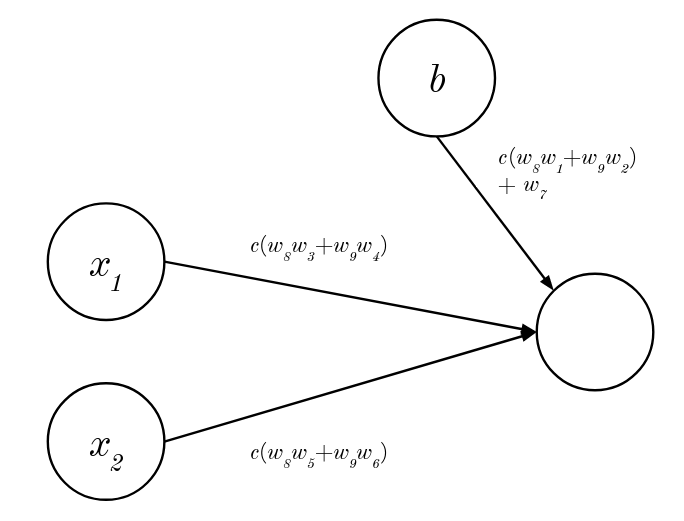
\includegraphics[width=\columnwidth]{net.png}

\section{Feature map sizes}
Dimension of the output is given as:
\begin{equation*}
	dim_{out} = \left\lceil\dfrac{dim_{in}-k+1+2p}{s}\right\rceil
\end{equation*}
\begin{enumerate}
	\item Input\\
		  $(300,300,3)$
	\item Layer 1\\
		  $7\times7$ conv; $30$. $s=2, p=0$\\
		  \begin{equation*}
		  dim_{out} = \left\lceil\dfrac{300-7+1+2(0)}{2}\right\rceil = 147
		  \end{equation*}
		  Layer 1 feature map size: $(147,147,30)$
	\item Layer 2\\
		  $3\times3$ maxpool. $s=2, p=0$\\
		  \begin{equation*}
		  dim_{out} = \left\lceil\dfrac{147-3+1+2(0)}{2}\right\rceil = 73
		  \end{equation*}
		  Layer 2 feature map size: $(73,73,30)$
	\item Layer 3\\
		  $3\times3$ conv; $50$. $s=1, p=3$\\
		  \begin{equation*}
		  dim_{out} = \left\lceil\dfrac{73-3+1+2(3)}{1}\right\rceil = 77
		  \end{equation*}
		  Layer 3 feature map size: $(77,77,50)$
\end{enumerate}
\end{document}